\documentclass[12pt]{third-rep}

%% Any characters from a % to the end of line are comments.

%% The third-rep class and this starter kit were written by 
%% Graham Gough <graham@cs.man.ac.uk>
%% If you have any comments or questions regarding this document,
%% please post them to the local newsgroup man.cs.tex.

%% This skeleton report is organised as a master file called
%% report.tex which then includes files for individual parts including
%% abstract.tex, chapter1.tex, chapter2.tex, chapter3.tex and
%% appendix1.tex.  

%% The third-rep style is a locally created style based on the
%% standard LaTeX report style. If you really want to have a look at
%% it, its source can be found in
%% /usr/local/share/texmf/tex/latex/mancs/third-rep.cls
%%
%% More information about LaTeX in general and the local setup in
%% particular can be found on the web at 
%% http://csis.cs.manchester.ac.uk/software/contrib/latex
%%
%%%%%%%%%%%%%%%%%%%%%%%%%%%%%%%%%%%%%%%%%%%%%%%%%%%%%%%%%%%%%%%%%%%%%%%%
%%
%% This is an example of how you load extra packages.
%% Some packages are already loaded in the third-rep class

\usepackage{url} % typeset URL's sensibly

\usepackage{pslatex} % Use Postscript fonts

%% The best way to latex just one chapter is to uncomment lines such as
%% the next:
%\includeonly{chapter1}

%% This defines the title (the \\ forces a line break)
\title{CSE221 Project}
%% and author
\author{Zhenchao Gan}
%% and the year of the report
\reportyear{2016}

%% The following line sets up the use of PostScript fonts rather
%% than the standard bitmapped fonts.
\usepackage{pslatex}

%% Uncomment the following line if you want to change the name of the
%% Bibliography to References
%\renewcommand{\bibname}{References}

\usepackage{listings}

%% End of preamble, the actual document starts here
%%


\newcommand{\horrule}[1]{\rule{\linewidth}{#1}} 	% Horizontal rule

\title{
		\vspace{-0.5in} 	
		\usefont{OT1}{bch}{b}{n}
		\normalfont \normalsize \textsc{University of California, San Diego \\
								Department of Computer Science and Engineering } \\ [25pt]
		\horrule{0.5pt} \\[0.4cm]
		\huge CSE 221 Project Report\\
		\horrule{2pt} \\[0.5cm]
}
\author{
		\normalfont 						\normalsize
        				Zhenchao Gan  (PID : A53092819)\\[-3pt]		\normalsize
				Di Huang (PID : A53081199)\\[-3pt]		\normalsize
        				Qiao Zhang (PID : A53095965)\\[-3pt]				\normalsize
				\{zhgan, dih024, qiz121\} @eng.ucsd.edu \\ \\
       		 \today
}
\date{}



\begin{document}

%% This actually creates the title and abstract pages
%\dotitleandabstract
\maketitle

\pagebreak

%% Generate contents etc
\tableofcontents

%% These include the actual text
\chapter{Introduction}
\label{cha:intro}


\section{Goal}
In this project, we will create and apply a set of experiments to Mac OS to characterize and understand its performance. The experiments are based on four aspects : 
\begin{enumerate}
\item CPU, Scheduling, and OS Services
\item Memory
\item Network
\item File System
\end{enumerate}


After the experiment, we will gain an intuitive feel for the relative speeds of different basic operations, which is invaluable in identifying performance bottlenecks.

\section{Environment}

\begin{itemize}
\item Language : C
\item Compiler : Configured with: --prefix=/Applications/Xcode.app/Contents/Developer/usr --with-gxx-include-dir=/usr/include/c++/4.2.1
Apple LLVM version 6.0 (clang-600.0.57) (based on LLVM 3.5svn)
Target: x86\_64-apple-darwin13.4.0
Thread model: posix
\item Optimization settings : no optimization set
\end{itemize}

\section{Time Estimation}
\begin{center}
\begin{tabular}{| c | c |}
\hline
Job &  Estimated Time   \\

\hline
Machine Description Collection & 6 hours \\  \hline
CPU, Scheduling, and OS Services Experiment & 15 hours \\  \hline
Memory Experiment & 10 hours \\  \hline
Network Experimentn & 10 hours \\  \hline
File System Experiment & 12 hours \\  \hline
Writing Report & 30 hours \\  \hline
Total & 83 hours \\  \hline

\end{tabular}
\end{center}

\chapter[Machine Description]{Machine Description}

\section{Processor}

I get this information through system profiler and command 
\begin{verbatim}
sudo sysctl -a | grep cache
\end{verbatim}

\begin{itemize}
\item Model : Intel Core i7
\item Cycle time : 0.4347826086 ns
\item L1 i-Cache : 32 KB
\item L1 d-Cache : 32KB
\item L2 Cache (per Core) : 256 KB
\item L3 Cache : 6 MB
\end{itemize}

\section{Memory}
I get this information by system profiler and run command
\begin{verbatim}
pagesize
\end{verbatim}

\begin{itemize}
\item Memory Bus Speed : 1600 MHz
\item RAM Size : 8 GB
\item Page Size : 4 KB
\end{itemize}

\section{I/O Bus}
\begin{verbatim}
sudo sysctl -a | grep busfrequency
\end{verbatim}

\begin{itemize}
\item Bus Frequency : 100 MHZ
\end{itemize}


\section{Disk}
I get this information from system profiler and simply measure IO.

\begin{verbatim}
 time dd if=/dev/zero bs=1024k of=tstfile count=1024
 dd if=tstfile bs=1024k of=/dev/null count=1024
\end{verbatim}

\begin{itemize}
\item Model : APPLE SSD SD256E
\item Capacity : 251 GB
\item RPM : I think RPM is no meaning to SSD
\item Controller Cache Size : 2 MB
\item File System : Journaled HFS+
\item Write Speed : 380 MB/s
\item Read Speed : 380 MB/s
\end{itemize}

\section{Network Card}
I get this information from system profiler.

\begin{itemize}
\item Card Type : AirPort Extreme
\item Network Card Speed : 450 Mbps
\end{itemize}

\section{Operating Systems}
I get this information from system profiler.

\begin{itemize}
\item OS : OS X, Version 10.9.5
\item Kern.ostype : Darwin
\item Kern.osrelease : 13.4.0
\end{itemize}

% Local Variables: 
% mode: latex
% TeX-master: "report"
% End: 

%\chapter{CPU, Scheduling, and OS Services}

\section{Measurement overhead}
In this part, we measure the overhead of reading time(read processor cycle counter) and the overhead of using a loop to measure many iterations of an operation. We will use these data to make other experiments more accurate by removing the overhead.

\paragraph{Methodology}
According to the hint, we googled rdtsc instruction and find useful helper functions rdtsc()\cite{rdtsc}, written in inline assembly form that return processor cycle count. 

In order to record the overhead of reading time, we call rdtsc() twice and subtract them. To measure the overhead of using a loop, we apply this method
\lstinputlisting[language=C]{hello.c}
We run it many times, and get the overhead by (end - start) / loops.

\paragraph{Predictions}
As for reading time, I guess the overhead of software is 8 cycles which I get from the inline assembly code. For the hardware layer, I guess it is 9 cycles to perform read, binary operation, write. So total 17 cycles for reading time; 

As for iterations of an operation, I guess software takes 3 cycles to do branch and increment and hardware takes 1 or 2 cycles as overhead, so it is about 5 cycles for iterations.

\paragraph{Results}
We present our measure results.

\begin{center}
\begin{tabular}{| p{2cm} | p{3cm} | p{3cm} | p{2cm} | p{3cm} | p{1cm} }
Operation  & Base Hardware Performance  & Estimated Software Overhead  & Predicted Time  & Measured Time  & Std  \\
\hline
Reading time & 9 cycles& 8 cycles& 17 cycles& 19.51327 cycles  & 1.9087  \\
Using a loop  & 2 cycles& 3 cycles& 5 cycles& 5.726476 cycles & 0.1728 \\
\end{tabular}
\end{center}

\paragraph{Discussion}
My prediction is pretty successful, very close to the measure value. Because we adopted low-overhead mechanism to measure operations and these operations are visible to use, we could follow and predict all the instructions they perform. So our prediction and methodology could get this result. 

\section{Procedure call overhead}
In this part, we measure the overhead of Procedure call. 

\paragraph{Methodology}
In order to get accurate result, we have to tell compiler not to inline the procedure call. So We use this attribute ((noinline)) to tell gcc not to inline procedure call and I turn off OPTIMIZE.

We did not process the arguments in procedure call. We iterate about 100000 times, I record the counter before the loop and record it again after the loop, then remove the iteration overhead.

\paragraph{Predictions}
We predicte when adding more arguments to procedure call, the cycle count should increase linearly. Because we should push each argument to the stack. Besides, procedure call will maintain stack pointers, and instruction like call and ret. When there are no arguments, the cycle should be about 6 cycles, 4 cycles for call, ret and maintain stack pointers and 2 cycles for hardware. When adding one more arguments, we assume hardware and software both add 1 cycles.


\paragraph{Results}
We present our measure results(unit : cycle).

\begin{center}
\begin{tabular}{l*{6}{c}r}
Args              & Hardware  & Software  & Overall  & Measured  & Remove overhead & Std\\
\hline
0 args & 2 & 4 & 6 & 7.1 & 2.1 & 0.16788\\
1 args & 3 & 5 & 8 & 7.3  & 2.3 & 0.19758 \\
2 args & 4 & 6 & 10 & 7.7 & 2.7 & 0.17281 \\
3 args & 5 & 7 & 12 & 8.6 & 3.6 & 0. 21230  \\
4 args & 6 & 8 & 14 & 9.3 & 4.3 & 0. 26652 \\
5 args & 7 & 9 & 16 & 10.0 & 5.0 & 0.17272 \\
6 args & 8 & 10 & 18 & 10.9 & 5.9 & 0.20281 \\
7 args & 9 & 11 & 20 & 13.1 & 8.1 & 0.22101 \\
\end{tabular}
\end{center}

\begin{figure}[htbp] %  figure placement: here, top, bottom, or page
   \centering
   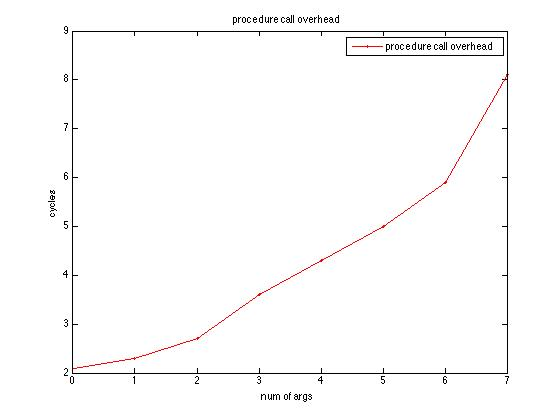
\includegraphics[width=5in]{./pics/pcall.jpg} 
   \caption{procedure call overhead}
   \label{fig:procedure call overhead}
\end{figure}

\paragraph{Discussion}
The measurement statistics is a little strange. Like we have predicted, the overhead for a procedure call scales about linearly with the number of arguments passed in; However, the cycles procedure calls take are less than we have predicted. 

So I tried another methodology. In a loop, first I record the counter, then do procedure call and record again. When calculating, I remove the overhead of counter reading time. But I still get similar results.

I have guessed that compiler may use registers to store parameter in the loop so as to reduce many memory operations. So I look at assembly code but it is pretty regular stack operation.

With the increasing of iteration time, the average cycles decrease a lot. There may be some mechanism like cache in the hardware.

\paragraph{Question} What is the increment overhead of an argument? The increment overhead is about 1 cycle per  argument, pushing parameters to stack.

\section{System call overhead}
In this part, we measure the overhead of System call. There are more than 100 systems in Mac OS and Linux like exit, fork, open and getpid. And the overhead varies a lot. For example, System call like fork will use more cycles than getpid. Because fork will creates a new process by duplicating the calling process which will use much more resources than getpid. So we aim to choose the one that use fewer CPU cycles. The minimal cost can be emulated by measuring the cost of getpid() or getppid().

\paragraph{Methodology}
Because in my operating system getpid() will cache the result. So we use a trick here. In each iteration, we fork a child process, and call getpid() in child process and then reap this child process. So every iteration we actually call getpid() in a bread-new  process, as a result we will never call getpid() on a cached one. So we solved this problem.

As before, we iterate about 100000 times, record the time before getpid() and after getpid(), then calculate the average cycles.

\paragraph{Predictions}
As for hardware, it may take 200 cycles to deal with registers. As for software, it is hard to estimate.  I know the operations including save current state to memory, trap into kernel, then kernel provide service and finally restore previous state. I measure it about 10000 cycles.

\paragraph{Results}
We present our measure results.

\begin{center}
\begin{tabular}{| p{2cm} | p{3cm} | p{3cm} | p{2.5cm} | p{2.5cm} | p{2cm}}
System call  & Base Hardware Performance  & Estimated Software Overhead  & Predicted Time  & Measured Time  & Std \\
\hline
getpid() & 200 cycles& 10000 cycles& 10200 cycles& 43020 cycles & 1702\\
\end{tabular}
\end{center}

\paragraph{Discussion}
Our estimates were lower than the measured result. That is to say, the overhead of user and kernel mode switch is more than we have imagined. So, caching some system call results may be a good idea. Because some stupid system call benchmark will repeatedly call getpid ().

\paragraph{Question} How does it compare to the cost of a procedure call? The cost of a system call is much larger than that of a procedure call. Because a system call involves switch between user mode and kernel mode. Furthermore, kernel will provide service to the caller and sometimes will have I/O operations.

\section{Task creation time}
In this part, we measure task creation time, measure the time to create and run both a process and a kernel thread.

\paragraph{Methodology}
For process, we use fork() to create a new process.  Each iteration we record time before fork(). Then there is a problem : Who executes first after fork(), parent or the child? In general, nothing can be said about the relative order of their execution. So we can not record time immediately after fork(). Here is our trick : in child process, we simply exit(); But in parent process, we use wait(NULL) and then record time. So after fork(), first parent process will give CPU to child process, then child process exit and kernel give CPU to parent process again. So there are two context switches. Then we subtract the two context switch overheads and get the final results. We run there procedure many times and get the average.

Things are quiet similar for kernel thread. We use pthread to create a task. Whenever we create a new thread, in the thread function we use pthread\_exit() to kill thread immediately, which will make measurement accurate.

\paragraph{Predictions}
It is difficult to predict accurately. What I am quiet sure is that creating a thread kernel is much more cheaper than creating a process. Because threads share many resources like file descriptors.

THOMAS E. ANDERSON in 1991 report it takes 11300 microseconds to fork process and 948 microseconds to create thread. \cite{task} In 1991, the CPU frequency of Intel 80486SX is 20MHz. Based on CPU frequency at that time, which are about 200000 cycles to fork process and 20000 cycles to create thread. So I do the following predictions.

For process, I guess the hardware overhead are 10000 cycles, and the software overhead is 190000 cycles.
For thread, I guess the hardware overhead are 1000 cycles, and the software overhead is 19000 cycles.

\paragraph{Results}
We present our measure results.

\begin{center}
\begin{tabular}{| p{2cm} | p{3cm} | p{3cm} | p{2.5cm} | p{2.5cm} | p{2cm} }
Task creation  & Base Hardware Performance  & Estimated Software Overhead  & Predicted Time  & Measured Time  & Std \\
\hline
process & 10000 cycles& 190000 cycles& 200000 cycles& 311751  cycles & 11321 \\
kernel thread    & 1000 cycles& 19000 cycles& 20000 cycles& 16509 cycles & 827\\
\end{tabular}
\end{center}

\paragraph{Discussion}
First, the cost of creating a process is much more expensive than a thread as the data indicated. Because thread is a light process that share many resources so it use fewer CPU cycles.

\paragraph{Question} How do they compare?
The cost of creating a new process is expensive. Each process has its own address space. Even with COW, there are still many memory copy operation and other overheads. Compared with process, kernel thread can share process resources and can be used in many situations. For example, in a web server, there are many clients and it is impossible to respond to so many clients using process creation model.

\section{Context switch time}
In this part, we measure the time to context switch from one process to another, and from one kernel thread to another.

\paragraph{Methodology}
As the hint indicated, blocking pipe will force context switch and we tried, it did do context switch so we use blocked pipe to perform context switch.

For process, we first record the time before read pipe, because read will block so it will switch to child process. Then we record the end time and write end time to pipe. So when parent process resume, parent process can collect the end time and do the calculation; Besides, we use wait() to reap resources.

For thread, we perform similar operations. After pthread\_create(), we record start time and use read to block pipe. At thread function we record the end time and write this value to pipe. So main thread could collect data and print the statistics.

At the end of each iteration, we all reap the resource in order to get accurate results. When there are many resources that are not reaped, our machine may run slower than usual.

\paragraph{Predictions}
What I am sure is that process context switch is much more expensive than thread context switch.

For process context switch, I think hardware cycles are 20000 cycles and software are 5000 cycles.

For thread context switch, I think hard cycles are 2000 cycles and software are 500 cycles.

\paragraph{Results}
We present our measure results.

\begin{center}
\begin{tabular}{| p{3cm} | p{3cm} | p{3cm} | p{3cm} | p{3cm} |}
Context switch              & Base Hardware Performance  & Estimated Software Overhead  & Predicted Time  & Measured Time   \\
\hline
process & 20000 cycles& 5000 cycles& 25000cycles & 133221 cycles \\
kernel thread    & 2000 cycles& 500 cycles& 2500 cycles& 9752 cycles\\
\end{tabular}
\end{center}

\paragraph{Discussion}
We predict well on the scale of process context switch and thread context switch. A process contains much more information than a kernel thread, so it is expensive of course just like previous experiments on creation time overhead.

The cost of process context switch is as expensive as fork a new process and so as a kernel thread. So context switch is very important to go deep into. How to reduce the overhead of context switch is of great significance.

\paragraph{Question} How do they compare?
In my experiment, kernel threads are approximately 14 times faster in performing a context switch than processes. So in some applications like web server, threads are much more cheaper than processes and recommended.
\chapter{Memory}

\section{RAM access time}
In this part, we report latency for individual integer accesses to main memory and the L1 and L2 caches.

\paragraph{Methodology}
To test memory access latency, I first followed the procedure described in the lmbench paper \cite{ramacc}, testing different stride lengths over varying sizes of arrays. 

Then I did not use normal array access, like A[i]. Because it may have other overheads. For example, the compiler may first calculate the address then access the element. Instead we use pointer access and store the next pointer in current variable. So we allocate an array of pointer of int, and each store the next element address.

\paragraph{Predictions}
Different level caches and main memory have different access cycles.

For L1-cache, we predict hardware cycles are 5 and software 2;
For L2-cache, we predict hardware cycles are 10 and software 4;
For L3-cache, we predict hardware cycles are 15 and software 6;
For main memory, we predict hardware cycles are 30 and software 10;

\paragraph{Results}
We present our measure results.

\begin{center}
\begin{tabular}{| p{1.5cm} | p{2cm} | p{2cm} | p{2cm} | p{2.5cm} | p{3cm} |}
TYPE             & Hardware  & Software  & Overall  & Measured  & Remove Overhead \\
\hline

L1	&   5 cycles  & 2 cycles & 7 cycles  &  7.5  cycles &  4.5 cycles \\
L2    &   10 cycles & 4 cycles & 14 cycles & 11.2 cycles &  8.2 cycles \\
L3 	&   15 cycles & 6 cycles & 21 cycles &  24.2 cycles & 21.2 cycles \\
Memory & 30 cycles & 10 cycles & 40 cycles & 200.3 cycles & 197.3 cycles \\
\end{tabular}
\end{center}


\begin {figure}
\centering
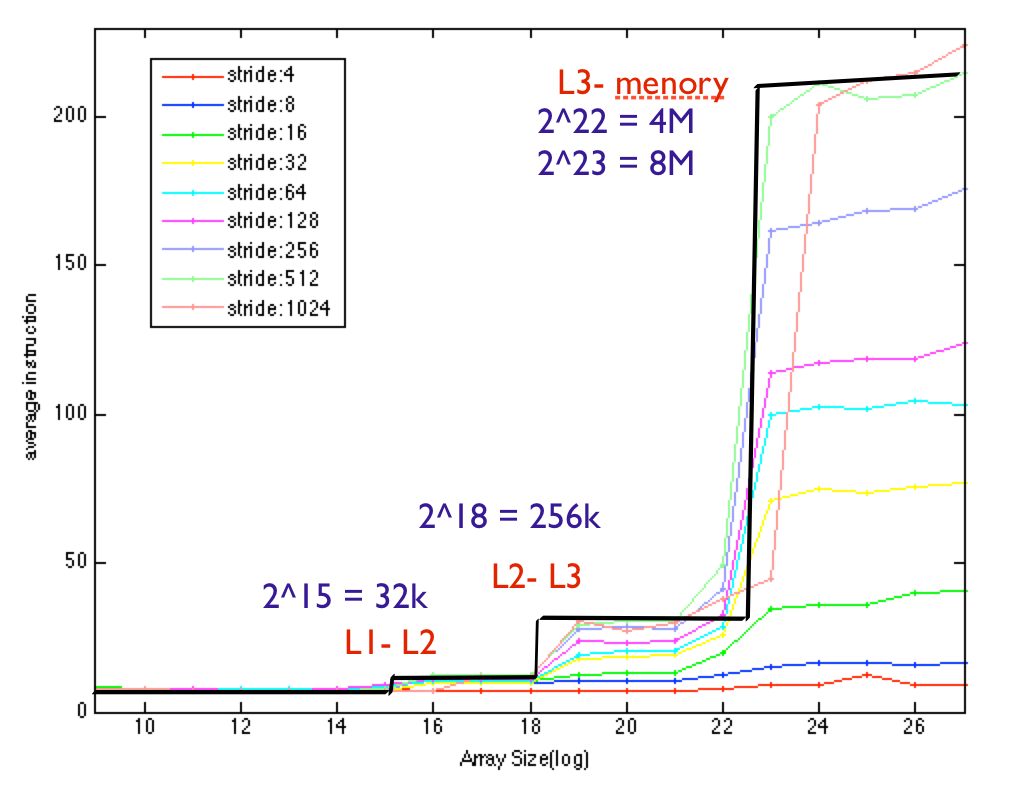
\includegraphics[width=2.6in]{./pics/ram1.png}
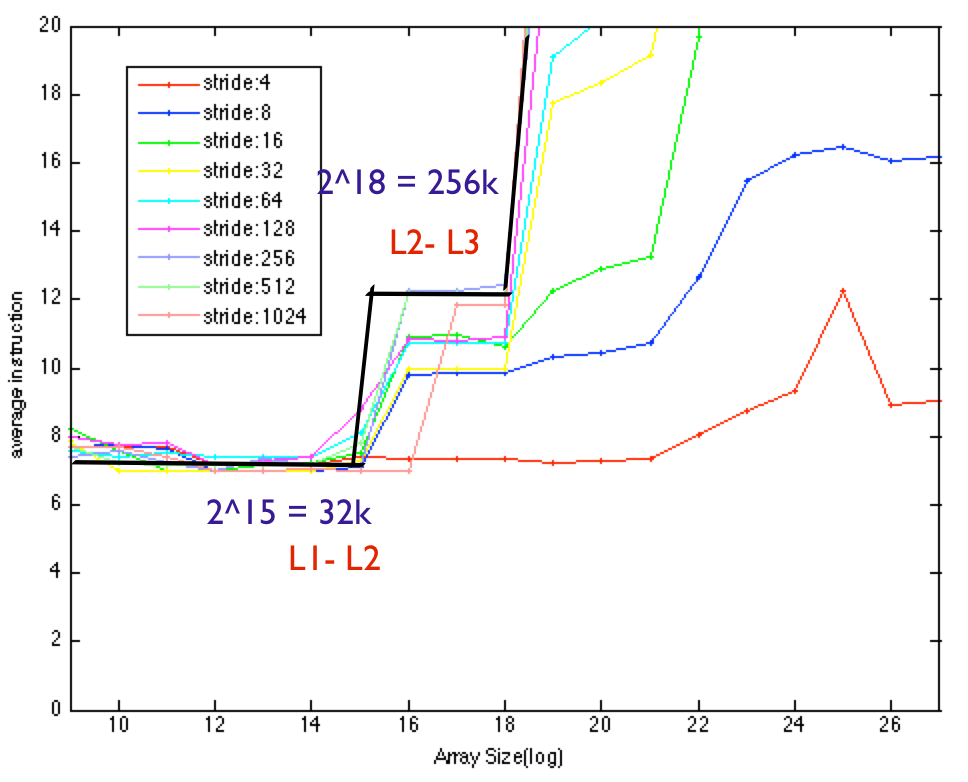
\includegraphics[width=2.6in]{./pics/ram2.png}
\caption{1,2}\label{RAM access}
\end{figure}


\paragraph{Discussion}
It is easy to see the transition from L3-cache to main memory, it is very steep in the picture from array size 22 to 23. Because my L3-cache is 6MB, so it is between 22 and 23.

We can also see the transitions from L2-cache to L3-cache. In the picture exactly in 18, the access time increase. Because my L2-cache is 256KB, which is equal to 18 in the picture.

In the scaled picture, it is very obvious to see transition from L1-cache to L2-cache, located in 15(32K).

We can also see that within cache, the RAM access time cycles are very small compared to that of main memory access.



\section{RAM bandwidth}
In this part, we report bandwidth for both reading and writing.

\paragraph{Methodology}
First, we create an array of size 32 MB that is bigger than L3-cache(6MB) and can be put into memory. In order to reduce the effects of cache line prefetching, we access array as follow : $0 -> HALF\_SIZE -> 1 -> HALF\_SIZE+1 -> ... -> ...$. So we can make sure that each access will cache miss and get from main memory.

To reduce the overhead, we apply loop unrolling. Compared with code that did not apply loop unrolling, the bandwidth increased  a lot.

\paragraph{Predictions}

I found an estimation about different RAM\cite{ramref}.

\begin{figure}[!htb]
\centering
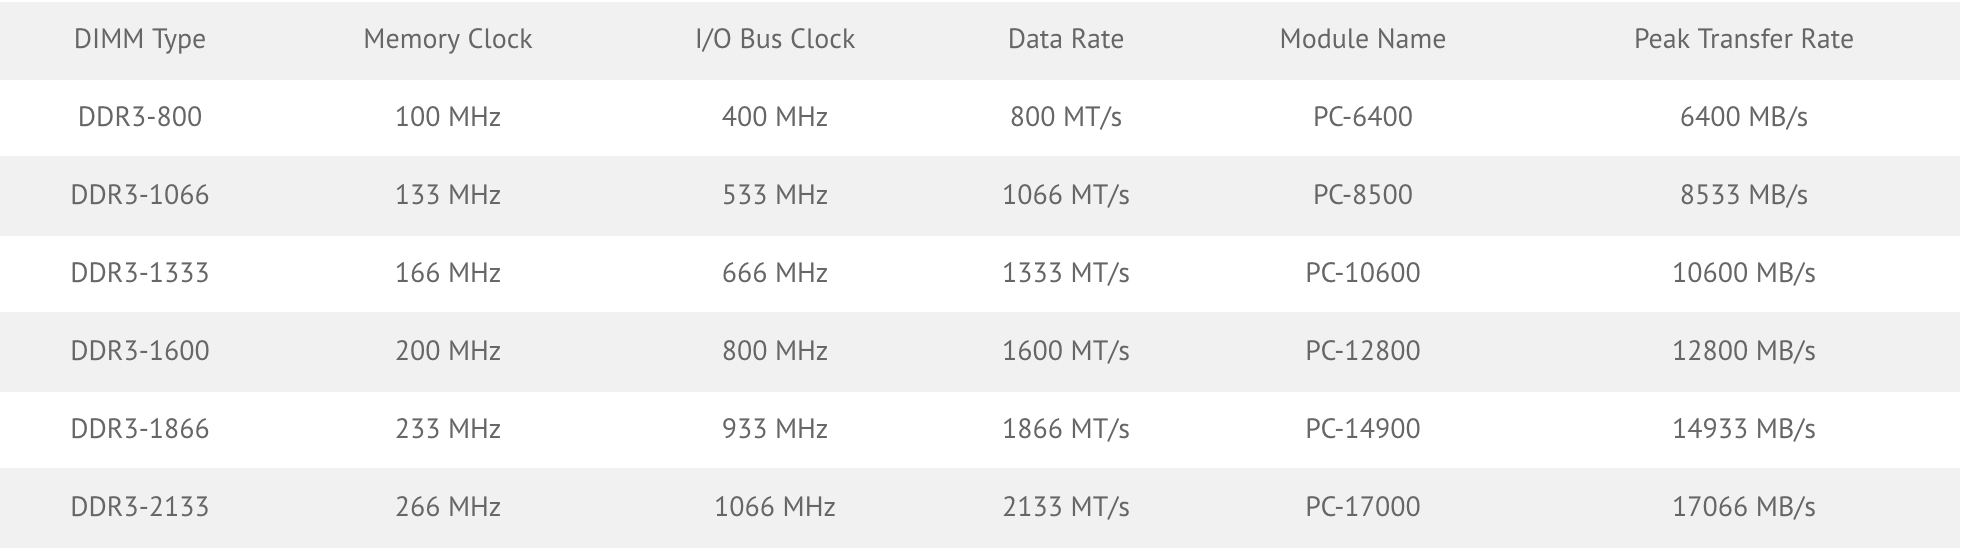
\includegraphics[width=6in]{./pics/ram_ref.png}
\caption{1}\label{RAM bandwidth}
\end{figure}

According to this article, the bandwidth of my machine should be 12800 MB/s. Besides, based on my hardware : 1600MHz RAM, it is should be 12800 MB/s.

\paragraph{Results}
We present our measure results.

\begin{center}
\begin{tabular}{l*{6}{c}r}
Operation             & Predicted Speed & Measured Speed & Std \\
\hline
READ & 12800MB/s & 8754MB/s & 99.49 \\
WRITE & 12800MB/s & 6902MB/s & 92.45\\

\end{tabular}
\end{center}

\paragraph{Discussion}
The prediction is a little higher than our measured results. 

Our method has eliminated the effects of cache line prefetching and use loop unrolling to reduce iteration overhead. That's why we choose 32MB array. Because an array of this size can not be put in cache totally and we can access array to make cache miss.

One of the drawback of our method is that we access each element of small size, which may include some overhead. If I have a big struct or class, maybe we can get higher results. 

\section{Page fault service time}
In this part, we report the time for faulting an entire page from disk.

\paragraph{Methodology}
According to the hint, we find that mmap is one useful mechanism. Because file contents are not read from disk initially and do not use physical RAM at all. The actual reads from disk are performed in a "lazy" manner, after a specific location is accessed. Before accessing the content, we record time, after accessing we record again then we can get the page fault service time.

\paragraph{Predictions}
According to some OS textbook \cite{page}, the page fault service time is about 8ms, the CPU frequency at that time is about 5MHz. So 8ms is about 16000 cycles.

Because my page size is 4 KB, every page fault will loading 4 KB data from disk to memory. SSD read/write speed is fast, so I predict the hardware overhead are 4096 * 2 = 8192 cycles and software overhead are 8000 cycles.

\paragraph{Results}
We present our measure results.

\begin{center}
\begin{tabular}{| p{3cm} | p{3cm} | p{3cm} | p{3cm} | p{3cm} |}
Operation  & Base Hardware Performance  & Estimated Software Overhead  & Predicted Time  & Measured Time   \\
\hline
Page Fault Service Time & 8192 cycles& 8000 cycles& 16192 cycles& 9898 cycles\\

\end{tabular}
\end{center}

\paragraph{Discussion}
Our estimation is a little higher than the measured result. Maybe today the hardware is much faster or the linux kernel serve page fault faster than that time.

Whenever the cpu detects a page-fault, its action depends on Current Privilege Level. If  CPL == 3  (executing in user mode)
the CPU will switch to its kernel-mode stack:

\begin{enumerate}
\item push  SS  and  ESP
\item push  EFLAGS
\item push  CS
\item push  EIP
\item push  error-code
\item jump to the page-fault service-routine  
\end{enumerate}

So there are a lot of work to do. 


\paragraph{Question} Dividing by the size of a page, how does it compare to the latency of accessing a byte from main memory?

The page size in our system is 4 KB, so it is approximately 1-2 cycles per byte of data transfered, compared to about 200 cycles per byte from main memory. May be this is the power of SSD.

%\chapter{Network}
In this chapter, the two machines are in the same LAN, with switch bandwidth about 1000Mb/s.

\section{Round trip time}
In this part, we try to measure the round trip time.

\paragraph{Methodology}
Our method is very simple, it's just like an echo server. Client send one byte to server, when server received the message then send back the message, then client receive it;
Before client send message, we record current cycle time; After client receive message, we record it again. We iterate this procedure for 1000 times and get the average result.


\paragraph{Predictions}
Our predictions exclude the factor of building connection. So for loopback and remote interface, the biggest difference is send and receive data.
For Ping program, we know that if use ICMP packet so it will get more accurate results. Because the ICMP requests are handled at the kernel level on the Linux side this will avoid two context switches.

Following is the Ping result.
\begin{center}
\begin{tabular}{l*{6}{c}r}
Operation       &  RTT \\
\hline
loopback & 0.070ms & 161000 cycles\\
remote & 0.196ms &  450800 cycles\\
\end{tabular}
\end{center}

Based on Ping results, we made our predictions.

For loopback interface. We expect the hardware overhead is 0.03ms, software overhead is 0.05ms.

For remote interface. We expect the hardware overhead is 0.2ms, software overhead is 0.05ms..

\paragraph{Results}
We present our measured results.

\begin{center}
\begin{tabular}{| p{2cm} | p{3cm} | p{3cm} | p{2cm} | p{2cm} | p{2cm}}
Operation   & Base Hardware Performance  & Estimated Software Overhead  & Predicted Time  & Measured Time  & Std \\
\hline
Loopback  & 0.03 ms& 0.05 ms& 0.08 ms & 0.04ms & 0.00725ms \\
Remote  & 0.2 ms& 0.05 ms & 0.25 ms & 0.27ms & 0.05ms \\ 
\end{tabular}
\end{center}

\paragraph{Discussion}
The overhead of network communication is large. Because TCP/IP protocol is implemented in kernel, so even the loopback results are a little slow for RTT. 

One weird thing is that for loopback interface, ICMP protocol is slower than TCP/IP protocol. It is weird that RTT measured by ICMP is longer than that measured by TCP/IP. One possible reason is that Ping program may did not use RDTSC instruction to measure time, losing some precision. \\

What can you deduce about baseline network performance and the overhead of OS software?  \\
In this experiment we only transfer several bytes of data. In the next experiment, we will go deep into the network performance and the overhead of OS software. Because bandwidth benchmark will reveal more about this. \\

How close to ideal hardware performance do you achieve? \\
It is far short of the ideal hardware performance because of the TCP/IP overhead.\\


What are reasons why the TCP performance does not match ideal hardware performance?  \\
First of all, normal TCP/IP protocols are implemented in kernel, so it is time-consuming to do context switch;
Secondly, We know there are many network stacks, from link layer to TCP/IP stacks;
Moreover, it is expensive to establish TCP connection, which will spend much time on handshake(like ACKs) to make sure the connection is reliable.

\section{Peak bandwidth}
In this part, we try to explore peak bandwidth.

\paragraph{Methodology}
The code is very similar to the previous experiment.

In this experiment, when we establish the connection, the client will send some data to the server and the server will receive this chunk of data. The size of data is a parameter. We have tried use different chunk sizes,  from 1MB to 64MB. The result is pretty similar. We add MSG\_WAITALL flag to recv() function. Because recv will immediately return if it detect there are some data in the buffer. So we add this flag to let recv() return if and only if it has received all the data.

We repeat this procedure 100 times and choose the maximum result as our peak bandwidth.

\paragraph{Predictions}
For the loopback device, the bottleneck will be the bandwidth of the RAM. Based on previous measured memory bandwidth : 8754MB/s, plus send and recv overhead, we predict the loopback peak bandwidth is about half of the measured memory bandwidth, that is about 4000 MB/s.

The network switch in my experiment is switching at the speed of 1000Mb/s, which is about 125MB/s. We except the switch to be the bottleneck. Considering TCP overhead, we decrease our prediction to 120MB/s.

\paragraph{Results}
We present our measured results.

\begin{center}
\begin{tabular}{l*{6}{c}r}
Operation       &  Predicted Speed& Measured Speed & Std\\
\hline
Loopback Peak Bandwidth & 4000 MB/s & 3328.38 MB/s & 132.65 MB/s\\
Remote Peak Bandwidth & 120 MB/s  & 114.82 MB/s & 2.72 MB/s\\
\end{tabular}
\end{center}


\paragraph{Discussion}
Our predictions are very close to the measured results. For loopback interface, the bandwidth speed is in the range [3GB/s, 4GB/s]; For remote interface, the speed is close to the switch bandwidth.

We also think the bandwidth can be influenced by many factors. For example, if the two machine are far from each other, then the route path is undecidable and the bandwidth will be influenced. \\

How close to ideal hardware performance do you achieve? \\
It is close to the hardware performance due to the perfect experiment environment.

\section{Connection overhead}
In this part, we try to explore connection overhead.

\paragraph{Methodology}
In this experiment, the client will connect to both the remote server and to the loopback interface 1000 times and we calculate the average.
We read the clock time before and after the corresponding system call and get the clock cycles.

\paragraph{Predictions}

Based on previous experience on RTT experiment and the network topology, we think  it would be 3-5 times higher than loopback interface. As for connection tear-down, we expect there is no big difference from connection setup.

Because TCP is a 3 way handshake protocol, we expect it is about 1.5-2.5 times of RTT.

\paragraph{Results}
We present our measured results.

\begin{center}
\begin{tabular}{| p{3cm} | p{3cm} | p{3cm} | p{2cm} | p{2cm} | p{2cm}}
Operation  & Base Hardware Performance  & Estimated Software Overhead  & Predicted Time  & Measured Time  & Std \\
\hline
Loopback Connection Setup & 0.0696ms & 0.0217ms & 0.0913ms & 0.133ms & 0.0112ms \\
Loopback Connection Tear-down & 0.0696ms & 0.0217ms & 0.0913ms & 0.0236ms & 0.0035ms \\
Remote Connection Setup & 0.391ms & 0.0217ms & 0.413ms & 0.271ms & 0.0179ms \\
Remote Connection Tear-down & 0.391ms & 0.0217ms & 0.413ms & 0.0614ms & 0.0048ms \\
\end{tabular}
\end{center}


\paragraph{Discussion}
Our predictions of connection tear-down are much higher than the measured results. It is very strange that it is so cheap to close the connection.
My guess is that maybe close works in asynchronous way.

%\chapter{File System}

\section{Size of file cache}
In this part, we try to determine the file cache size.

\paragraph{Methodology}
If the file the fit into cache totally, then it would be very fast to read. If the file is too big that can not be put into cache totally, then read would be slower then that fir into cache totally. 

So I prepared 40 files with different sizes ranging from 1GB to 4GB. We read each file 10 times and calculate  read cycles/MB.

\paragraph{Predictions}
Our computer main memory is 8GB. So the cache must be less than 8GB; Besides, the project web page says it is a notable fraction of main memory and can be several GBs. So we predict it is 2GBs.

\paragraph{Results}
We present our measure results. By the way, we only include result from 3GB to 4GB, because the cache size is in this range.

\begin{center}
\begin{tabular}{l*{6}{c}r}
File Size             &  Cycles/MB\\
\hline
3000MB & 610 \\
3100MB & 614 \\
3200MB & 598 \\
3300MB & 622 \\
3400MB & 1965 \\
3500MB & 5498 \\
3600MB & 5572 \\
3700MB & 5503 \\
3800MB & 5673 \\
3900MB & 5657 \\
4000MB & 5598 \\

\end{tabular}
\end{center}

\begin{figure}[htbp] %  figure placement: here, top, bottom, or page
   \centering
   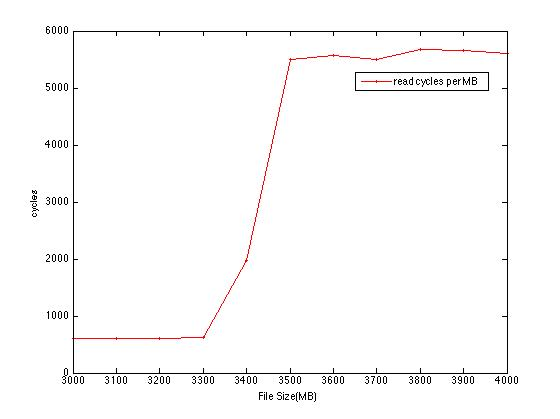
\includegraphics[width=5in]{./pics/41.jpg} 
   \caption{read cycles}
   \label{fig:read cycles}
\end{figure}

\paragraph{Discussion}
The graph shows that the file cache size is between 3300MB and 3500MB. Before this experiment, I did not realize that OS will use so many spaces for file cache. This optimisation speed up file reading time.

\section{File read time}
In this part, we report for both sequential and random access as a function of file size.

\paragraph{Methodology}
First, in order not to measure cached data, we want to set O\_DIRECT flag when opening a file, which could minimize cache effects of the I/O from this file. But Mac OS does not support O\_DIRECT. So we looked through Apple document and find we can set F\_NOCACHE in fcntl().

Besides, we use read() for sequential access, because read() will modify file pointer that fit the situation; However for random access it is bad to use read(), because we have to use lseek() to move the file pointer to target position which will significantly cost time. So we use pread() instead of read() for random access. Pread() works just like read() but reads from the specified position in the file without modifying the file pointer.

We provide several files with different sizes and iterate 100 times, then calculate  the average per-block read time.

\paragraph{Predictions}
Because we are using SSD, the speed of sequential and random access may be very similar to each other. Considering that we did not use file cache, we will fetch each block of data from disk. So I predict the speed is 19000 cycles per blocks, plus 1000 cycles for software.

\paragraph{Results}
We present our measure results. The base file is 4KB, and we define log(4KB) = 2.

\begin{figure}[htbp] %  figure placement: here, top, bottom, or page
   \centering
   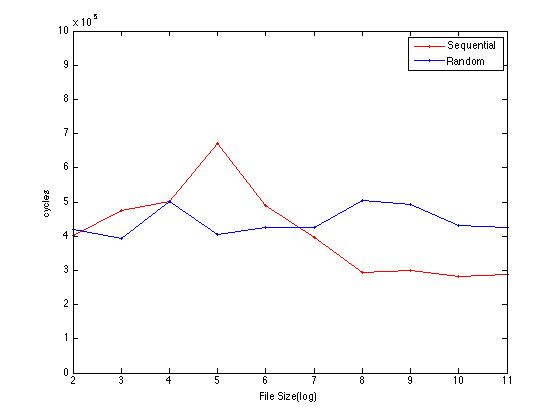
\includegraphics[width=5in]{./pics/42.jpg} 
   \caption{read cycles per block}
   \label{fig:read cycles per block}
\end{figure}

\begin{center}
\begin{tabular}{| p{4cm} | p{2.5cm} | p{2.5cm} | p{2.5cm} | p{2.5cm} |}
File Size &  Base Hardware Performance  & Estimated Software Overhead  & Predicted Time  & Measured Time   \\

\hline
4KB & 19000 cycles& 1000 cycles& 20000 cycles& 401481 cycles\\ 
8KB & 19000 cycles& 1000 cycles& 20000 cycles& 475677 cycles\\ 
16KB & 19000 cycles& 1000 cycles& 20000 cycles& 501356 cycles\\
32KB & 19000 cycles& 1000 cycles& 20000 cycles& 670260 cycles\\
64KB & 19000 cycles& 1000 cycles& 20000 cycles& 489722 cycles\\
128KB & 19000 cycles& 1000 cycles& 20000 cycles& 397495 cycles\\
256KB & 19000 cycles& 1000 cycles& 20000 cycles& 293712 cycles\\
512KB & 19000 cycles& 1000 cycles& 20000 cycles& 300106 cycles\\
1024KB & 19000 cycles& 1000 cycles& 20000 cycles& 281106 cycles\\
2048KB & 19000 cycles& 1000 cycles& 20000 cycles& 287629 cycles\\

\end{tabular}
\end{center}

Above is the result of sequential access. We can see on average it takes about 300000-600000 cycles to read each file block, far exceeding than we predicted previously.

\begin{center}
\begin{tabular}{| p{4cm} | p{2.5cm} | p{2.5cm} | p{2.5cm} | p{2.5cm} |}
File Size   & Base Hardware Performance  & Estimated Software Overhead  & Predicted Time  & Measured Time   \\
\hline
4KB & 19000 cycles& 1000 cycles& 20000 cycles& 420067 cycles\\ 
8KB & 19000 cycles& 1000 cycles& 20000 cycles& 393597 cycles\\ 
16KB & 19000 cycles& 1000 cycles& 20000 cycles& 502322 cycles\\
32KB & 19000 cycles& 1000 cycles& 20000 cycles& 405538 cycles\\
64KB & 19000 cycles& 1000 cycles& 20000 cycles& 425528 cycles\\
128KB & 19000 cycles& 1000 cycles& 20000 cycles& 426442 cycles\\
256KB & 19000 cycles& 1000 cycles& 20000 cycles& 504624 cycles\\
512KB & 19000 cycles& 1000 cycles& 20000 cycles& 492654 cycles\\
1024KB & 19000 cycles& 1000 cycles& 20000 cycles& 430804 cycles\\
2048KB & 19000 cycles& 1000 cycles& 20000 cycles& 426658 cycles\\

\end{tabular}
\end{center}

Above is the result of random access. We can see on average it takes about 400000-500000 cycles to read each file block, far exceeding than we predicted previously.

\paragraph{Discussion}
As we have predicted, random access is almost as fast as sequential access due to SSD. But we predict cycles wrongly. Without file cache, it would be very expensive to do file reading. Each block would cost almost 300000-600000 cycles on average.

Then I remove F\_NOCACHE flag to do file reading, finding that it only takes about 1000-2000 cycles per block, which is so cheap compared with no cache. It speeds up over 100 times. So, in most situations open file with cache is good for program performance.

\section{Remote file read time}
In this section, we conduct the previous experiment for a remote file system.

\paragraph{Methodology}
We use the same method described in previous section. The only difference is that we now read a remote file. Note, page size in that machine is 8KB.

\paragraph{Predictions}
The remote machine use SSD, and the network bandwidth is 1000Mb/s, these two machines are in same LAN. So the effect of network may not seem so obvious.

Based on the results of previous section, we add 20\% overhead in hardware and software. Don't forget that the pagesize now is 8KB. And we think sequential access time is close to random access time. 

\paragraph{Results}

We present our measure results. The base file is 4KB, and we define log(4KB) = 2.

\begin{figure}[htbp] %  figure placement: here, top, bottom, or page
   \centering
   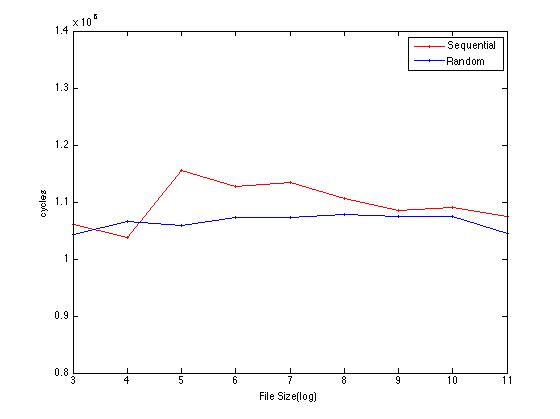
\includegraphics[width=4in]{./pics/43.jpg} 
   \caption{remote read cycles per block}
   \label{fig:remote read cycles per block}
\end{figure}

\begin{center}
\begin{tabular}{| p{4cm} | p{2.5cm} | p{2.5cm} | p{2.5cm} | p{2.5cm} |}
File Size  & Base Hardware Performance  & Estimated Software Overhead  & Predicted Time  & Measured Time   \\
\hline
8KB & 800000 cycles& 10000 cycles& 810000 cycles& 1060023 cycles\\ 
16KB & 800000 cycles& 10000 cycles& 810000 cycles& 1037613 cycles\\ 
32KB & 800000 cycles& 10000 cycles& 810000 cycles& 1155908 cycles\\
64KB & 800000 cycles& 10000 cycles& 810000 cycles& 1127454 cycles\\
128KB & 800000 cycles& 10000 cycles& 810000 cycles& 1134455 cycles\\
256KB & 800000 cycles& 10000 cycles& 810000 cycles& 1105819 cycles\\
512KB & 800000 cycles& 10000 cycles& 810000 cycles& 1085479 cycles\\
1024KB & 800000 cycles& 10000 cycles& 810000 cycles& 1089600 cycles\\
2048KB & 800000 cycles& 10000 cycles& 810000 cycles& 1074542 cycles\\

\end{tabular}
\end{center}

Above is the result of sequential access.

\begin{center}
\begin{tabular}{| p{4cm} | p{2.5cm} | p{2.5cm} | p{2.5cm} | p{2.5cm} |}
File Size  & Base Hardware Performance  & Estimated Software Overhead  & Predicted Time  & Measured Time   \\
\hline
8KB & 800000 cycles& 10000 cycles& 810000 cycles& 1043427 cycles\\ 
16KB & 800000 cycles& 10000 cycles& 810000 cycles& 1065662 cycles\\ 
32KB & 800000 cycles& 10000 cycles& 810000 cycles& 1058558 cycles\\
64KB & 800000 cycles& 10000 cycles& 810000 cycles& 1073499 cycles\\
128KB & 800000 cycles& 10000 cycles& 810000 cycles& 1073262 cycles\\
256KB & 800000 cycles& 10000 cycles& 810000 cycles& 1077349 cycles\\
512KB & 800000 cycles& 10000 cycles& 810000 cycles& 1074041 cycles\\
1024KB & 800000 cycles& 10000 cycles& 810000 cycles& 1074543 cycles\\
2048KB & 800000 cycles& 10000 cycles& 810000 cycles& 1044684 cycles\\

\end{tabular}
\end{center}

Above is the result of random access.

\paragraph{Discussion}
Due to previous experience, this time our estimation is very close to the measured results. And it seems that the overhead is not so much compared with file cache. If one machine is in China, another one is in US, maybe network is very expensive compared to other factors.

SSDs also make random access as fast as sequential access.

\paragraph{Question} What is the "network penalty" of accessing files over the network?  As we have predicted, compared with file cache, the network overhead is about 20\%, around 200000 cycles.

\section{Contention}
In this section, we report the average time to read one file system block of data as a function of the number of processes simultaneously performing the same operation on different files on the same disk (and not in the file buffer cache).

\paragraph{Methodology}
As previous experiment, we continue using F\_NOCACHE flag to disable file cache. In this experiment, we create several processes. Each process read different file which is of the same size : 1MB. And we iterate 100 times to get average data. 

\paragraph{Predictions}
We are sure that the more process number, the more cycles it spend on reading file. We think each read will result in a context switch to another process. We present predictions with results in the following table. We use 1MB file, including 256 blocks. Based on previous experiment on sequential reading 1MB file, when there is only 1 process, the reading cycles are 281106. When increasing a process, we add about 15000 cycles for hardware and 1000 for software.

\paragraph{Results}
We present our measure results.

\begin{center}
\begin{tabular}{| p{4cm} | p{2.5cm} | p{2.5cm} | p{2.5cm} | p{2.5cm} |}
nprocesses   & Base Hardware Performance  & Estimated Software Overhead  & Predicted Time  & Measured Time   \\
\hline
1 & 280000 cycles& 1000 cycles& 281000cycles & 229003 cycles\\
2 & 295000 cycles& 2000 cycles& 297000 cycles& 253880 cycles\\
3 & 310000 cycles& 3000 cycles& 313000 cycles& 209028 cycles\\
4 & 325000 cycles& 4000 cycles& 329000 cycles& 240578 cycles\\
5 & 340000 cycles& 5000 cycles& 345000 cycles& 432147 cycles\\
6 & 355000 cycles& 6000 cycles& 371000 cycles& 438801 cycles\\
7 & 370000 cycles& 7000 cycles& 377000 cycles& 459831 cycles\\
8 & 385000 cycles& 8000 cycles& 393000 cycles& 415745 cycles\\
9 & 400000 cycles& 9000 cycles& 409000 cycles& 474147 cycles\\
10 & 415000 cycles& 10000 cycles& 425000 cycles& 491004 cycles\\
11 & 430000 cycles& 11000 cycles& 441000 cycles& 515341 cycles\\
12 & 445000 cycles& 12000 cycles& 457000 cycles& 515871 cycles\\
13 & 460000 cycles& 13000 cycles& 473000 cycles& 536629 cycles\\
14 & 475000 cycles& 14000 cycles& 489000 cycles& 568728 cycles\\
15 & 490000 cycles& 15000 cycles& 505000 cycles& 590147 cycles\\

\end{tabular}
\end{center}

\begin{figure}[htbp] %  figure placement: here, top, bottom, or page
   \centering
   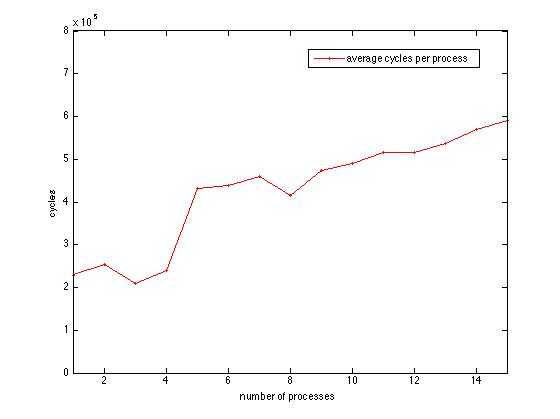
\includegraphics[width=4.5in]{./pics/44.jpg} 
   \caption{average cycles per process}
   \label{fig:average cycles per process}
\end{figure}

\paragraph{Discussion}
We can see that generally, with the increasing of process, the average cycle increase too. 

Our prediction is so close to the measured results. I am very surprised, I had thought that the measured results may exceed millions of cycles due to context switch between processes.

When I set the file cache flag, the cycles reduce to about 6000-8000 per block.

If we use HDD, each read will take many seek time. Now we use SSD, the cost is very small. That's the big difference between SSD and HDD.

\bibliography{refs}             % this causes the references to be
                                % listed

\bibliographystyle{alpha}       % this determines the style in which
                                % the references are printed, other
                                % possible values are plain and abbrv
%% Appendices start here
%\appendix
\chapter{Summary}

\small
\begin{center}
\begin{tabular}{| p{4cm} | p{2cm} | p{2cm} | p{2cm} | p{2.5cm} | p{2cm} }
\hline
Operation  & Base Hardware Performance  & Estimated Software Overhead  & Predicted Time  & Measured Time  & Std \\
\hline 
CPU & & & & &\\
\hline
Reading time & 9 cycles & 8 cycles & 17 cycles & 19.51327 cycles & 1.9087\\
Loop overhead & 2 cycles& 3 cycles& 5 cycles& 5.726476 cycles & 0.1728 \\
System call & 200 cycles& 10000 cycles& 10200 cycles& 43020 cycles & 1702 \\
Task creation : process & 10000 cycles& 190000 cycles& 200000 cycles& 311751 cycles & 11321\\
Task creation : kernel thread    & 1000 cycles& 19000 cycles& 20000 cycles& 16509 cycles & 827\\
Context switch : process & 20000 cycles& 5000 cycles& 25000 cycles& 133221  cycles & 3428\\
Context switch : kernel thread    & 2000 cycles& 500 cycles& 2500 cycles& 9752 cycles & 439\\
\hline 
Memory & & & & &\\
\hline
RAM Access Time : L1 Cache (64KB) &   5 cycles  & 2 cycles & 7 cycles &  4.5 cycles & 0.1212 \\
RAM Access Time : L2 Cache (256KB) & 10 cycles & 4 cycles & 14 cycles &  8.2 cycles & 0.2059\\
RAM Access Time : L3 Cache (6MB) & 15 cycles & 6 cycles & 21 cycles  & 21.2 cycles & 0.4529\\
RAM Access Time : Main Memory (8G) & 90 cycles & 60 cycles & 150 cycles & 197.3 cycles & 6.2800\\
RAM Read Bandwidth & & & 12800MB/s & 8754MB/s & 99.49 \\
RAM Write Bandwidth & & & 12800MB/s & 6902MB/s & 92.45\\
Page Fault Service Time & 8192 cycles& 8000 cycles& 16192 cycles& 8528 cycles & 11.33405\\
\end{tabular}
\end{center}

\small
\begin{center}
\begin{tabular}{| p{4cm} | p{2cm} | p{2cm} | p{2cm} | p{2.5cm} | p{2cm}} 

\hline 
Network & & & & & \\
\hline
Loopback RTT & 0.01 ms & 0.05 ms& 0.06 ms & 0.03ms & 0.00725ms \\
Remote RTT & 0.05 ms& 0.2 ms & 0.25 ms & 0.27ms & 0.05ms\\
Loopback Peak Bandwidth & & & 1600 MB/s & 1540 MB/s \\
Remote Peak Bandwidth & & &  125 MB/s  & 133 MB/s\\
Loopback Connection Setup & 35000 cycles& 5000 cycles& 40000 cycles& 306665 cycles \\
Loopback Connection Tear-down & 20000 cycles& 3000 cycles& 23000 cycles& 54334 cycles \\
Remote Connection Setup & 300000  cycles& 30000 cycles& 330000 cycles& 622923 cycles\\
Remote Connection Tear-down & 150000  cycles& 15000 cycles& 165000 cycles& 141333 cycles\\

\hline 
File System& & & & \\
\hline
File Cache Size & & & 2GB & 3.3GB \\ 
Sequential File Read Time Per Block& 19000 cycles & 1000 cycles& 20000 cycles& 300106 cycles & 10085 cycles\\
Random File Read Time Per Block& 19000 cycles& 1000 cycles& 20000 cycles& 492654 cycles & 12320 cycles \\
Sequential Remote File Read Time Per Block& 800000 cycles& 10000 cycles& 810000 cycles& 1089600 cycles & 20334 cycles\\
Random Remote File Read Time Per Block& 800000 cycles& 10000 cycles& 810000 cycles& 1074543 cycles & 10004 cycles\\
File Contention(15 processes) & 490000 cycles& 15000 cycles& 505000 cycles& 590147 cycles & 25980 cycles \\

\end{tabular}
\end{center}
\end{document}